\chapter{Two-source high harmonic generation}
\label{two_source}

\section{Introduction}
\label{intro_ts}

A common difficulty in working with extreme ultraviolet (XUV) light is the lack of efficient and broadband optics, especially beam splitters. In this chapter, I will introduce a method for generating two sources of XUV light by high harmonic generation using a \gls{swpg}.  This \gls{swpg} allows for the duplication of an \gls{ir} pulse, as well as precise and stable control of the relative phase between the duplicates of the input \gls{ir} pulse. The two most intense duplicates can generate harmonics which will interfere in the far-field. This can be thought of as an inline Mach-Zehnder interferometer with interferometric stability on sub-wavelength level of the high harmonic. The inherent stability of this two-source scheme will be utilized to measure both the real and imaginary parts of the refractive index of a medium.

\section{Theory}
\subsection{Laser beam shaping using diffractive optics}
\label{theory_ts}
%Describe general problem of beam shaping using DOEs. see \cite{romeroMathematicalAspectsLaser2010,romeroMathematicalTheoryLaser2010,romeroTheoryOptimalBeam2007}
In many experimental designs, it is advantageous to be able to shape the spatial intensity distribution of light to be something other than a typical Gaussian beam.  Furthermore, this control over the intensity distribution is ideally done in such a way that is, at least in principle, lossless.  This can be achieved by introducing a \gls{doe} which spatially shapes the phase of an incoming pulse.  A simple and general schematic of this is shown in figure  \ref{beam_shaping_scheme}.  The idea is simple, by introducing a particular spatially dependent phase $P(x, y)=e^{i\phi(x, y)}$, one is able to produce the design intensity distribution at the focal plane of the lens.


\subsection{Beam splitting grating}
\subsection{Imperfect phase grating}
\section{Two-source high harmonic generation}


\begin{equation}\label{eq:field}
	S(x) = \sum_{n} E(x - x_{n})
\end{equation}

\begin{figure}
	\centering
	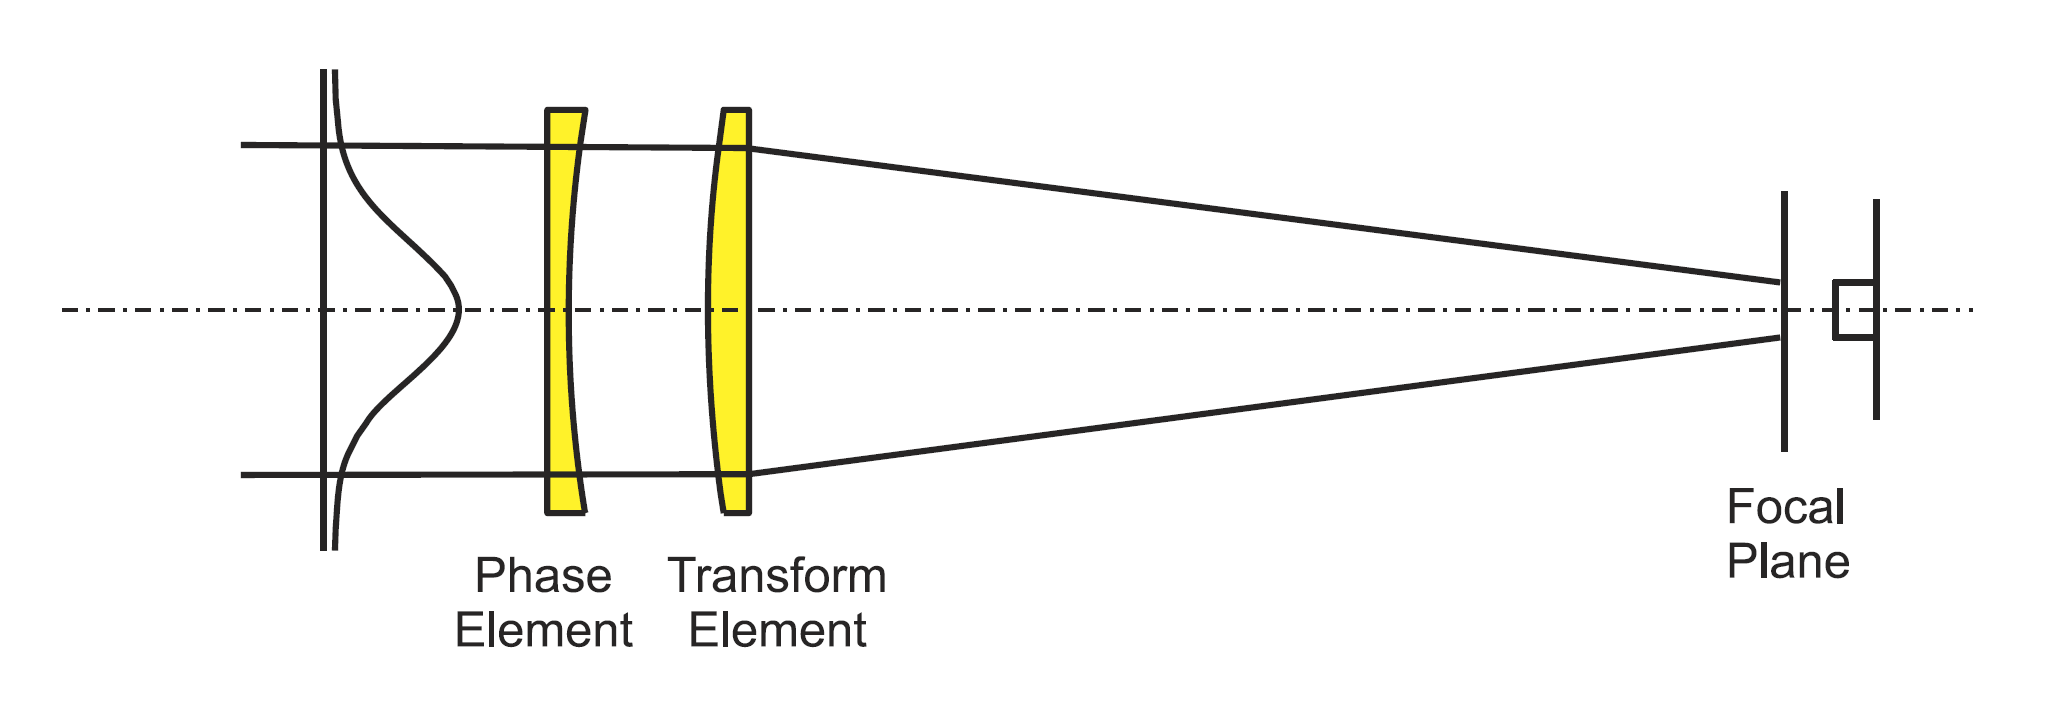
\includegraphics[width=0.9\textwidth]{figures/Two_source/romero_beam_shaping_schematic.png}
	\caption{Schematic demonstrating how to use a diffractive optical element to shape the beam profile at the focal plane. A collimated coherent beam is incident upon a diffractive optical element which shapes the phase of the incident beam, and then a lens is used as a transform element to Fourier transform the beam at the focal plane.  The intensity profile at the focal plane can be controlled by altering the spatial dependence of the phase imparted upon the incident beam by the phase element. Adapted from \cite{romeroMathematicalAspectsLaser2010}}
	\label{beam_shaping_scheme}
\end{figure}


\begin{figure}
	\centering
	\begin{subfigure}[b]{0.45\textwidth}
		\caption{}
		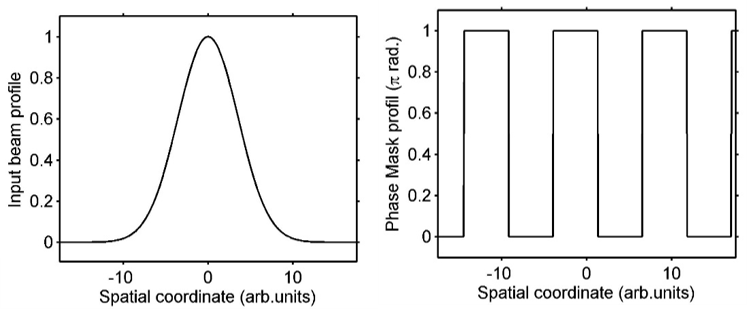
\includegraphics[width=\textwidth]{figures/Two_source/spatial_profile}
		\label{fig:spatial_profile}
	\end{subfigure}
	\begin{subfigure}[b]{0.45\textwidth}
		\caption{}
		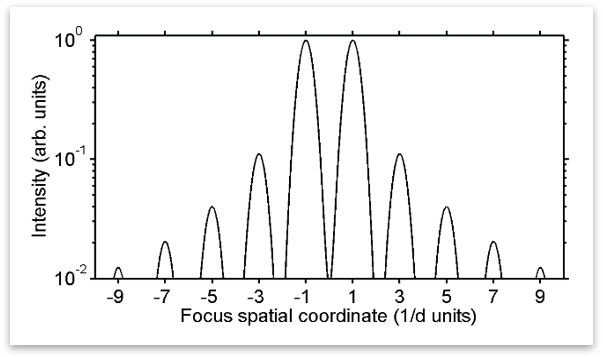
\includegraphics[width=\textwidth]{figures/Two_source/focus_profile}
		\label{fig:focus_profile}
	\end{subfigure}
	\caption{(a) Two-channel model for Feshbach resonance.  Incident atoms in the entrance channel (the open channel) couple to a bound state of energy $E_{c}$ supported by the closed channel.  Since collisions take place for $E\rightarrow 0$, tuning $E_{c}$ to 0 allows for the resonant coupling to occur. (b) Scattering length near a resonance where a bound state crosses the scattering threshold. Inset shows the quadratic behavior of the binding energy near the resonance.}
\end{figure}


\begin{equation}
	\begin{aligned}
    	I_{IR} &= a + b\times\cos\left(\phi(x_{0})\right)\\
     	I_{q} &= \alpha_q\times a^{q} \left(1+N_{q}\frac{b}{a}\cos\left(\phi(x_{0})\right)\right) + o(b\times a^{q-1})\\
	\end{aligned}
\end{equation}
\begin{equation}
	\begin{aligned}
		I_{IR}(\tilde{x}_{1},x_{0}) &= \left|\tilde{S}(\tilde{x}_{1},x_{0})\right|^{2} \\
		&= \left|a_{-1}\tilde{E}(2\tilde{x}_{1})+a_{0}\tilde{E}(\tilde{x}_{1})+a_{1}\tilde{E}(0)+a_{3}\tilde{E}(2\tilde{x}_{1})\right|^{2}\\
     &= \left|a_{0}\tilde{E}(\tilde{x}_{1})+a_{1}\tilde{E}(0)\right|^{2}\\
	\end{aligned}
\end{equation}
\begin{equation}
	\begin{aligned}
		 I_{IR}(\tilde{x}_{1},x_{0}) &=\left|\tilde{E}(0)\right|^{2}\left|\frac{2}{\pi}\sin\left(\xi\frac{\pi}{2}\right)e^{i(\xi\frac{\pi}{2}-\phi_{1})}+\cos\left(\xi\frac{\pi}{2}\right)e^{i\xi\frac{\pi}{2}}\frac{\tilde{E}(\tilde{x}_{1})}{\tilde{E}(0)} -  \frac{2\sin\left(\xi\frac{\pi}{2}\right)}{\pi}e^{i(\xi\frac{\pi}{2}+\phi_{1})}\frac{\tilde{E}(2\tilde{x}_{1})}{\tilde{E}(0)} + \frac{2\sin\left(\xi\frac{\pi}{2}\right)}{3\pi}e^{i(\xi\frac{\pi}{2}-3\phi_{1})}\frac{\tilde{E}(2\tilde{x}_{1})}{\tilde{E}(0)}\right|^{2}\\
	\end{aligned}
\end{equation}
\begin{equation}
	\begin{aligned}
		I_{IR}(\tilde{x}_{1},x_{0})  &= \left|\tilde{E}(0)\frac{2}{\pi}\sin\left(\xi\frac{\pi}{2}\right)\right|^{2}\left|e^{-i\phi_{1}}+\frac{\pi}{2\tan\left(\xi\frac{\pi}{2}\right)}\frac{\tilde{E}(\tilde{x}_{1})}{\tilde{E}(0)} -e^{i\phi_{1}}\frac{\tilde{E}(2\tilde{x}_{1})}{\tilde{E}(0)} +  \frac{e^{-3i\phi_{1}}}{3}\frac{\tilde{E}(2\tilde{x}_{1})}{\tilde{E}(0)}\right|^{2}\\
		&= \left|\tilde{E}(0)\frac{2}{\pi}\sin\left(\xi\frac{\pi}{2}\right)\right|^{2}\left(1+\frac{\pi}{\tan\left(\xi\frac{\pi}{2}\right)}\frac{\tilde{E}(\tilde{x}_{1})}{\tilde{E}(0)}\cos(\phi_{1})-\frac{4}{3}\frac{\tilde{E}(2\tilde{x}_{1})}{\tilde{E}(0)}\cos(2\phi_{1})\right)\\
		I_{IR}(\tilde{x}_{-1},x_{0}) &= \left|\tilde{S}(\tilde{x}_{-1},x_{0})\right|^{2} \\
		 &= \left|a_{-1}\tilde{E}(0)+a_{0}\tilde{E}(\tilde{x}_{1})\right|^{2}\\
		&= \left|\tilde{E}(0)\right|^{2}\left|-\frac{2}{\pi}\sin\left(\xi\frac{\pi}{2}\right)e^{i(\xi\frac{\pi}{2}+\phi_{1})}+\cos\left(\xi\frac{\pi}{2}\right)e^{i\xi\frac{\pi}{2}}\frac{\tilde{E}(\tilde{x}_{1})}{\tilde{E}(0)}+\frac{2\sin\left(\xi\frac{\pi}{2}\right)}{\pi}e^{(\xi\frac{\pi}{2}-\phi_{1})}\frac{\tilde{E}(2\tilde{x}_{1})}{\tilde{E}(0)} -  \frac{2\sin\left(\xi\frac{\pi}{2}\right)}{3\pi}e^{(\xi\frac{\pi}{2}+3\phi_{1})}\frac{\tilde{E}(2\tilde{x}_{1})}{\tilde{E}(0)}\right|^{2}\\
      &= \left|\tilde{E}(0)\frac{2}{\pi}\sin\left(\xi\frac{\pi}{2}\right)\right|^{2}\left|e^{-i\phi_{1}}-\frac{\pi}{2\tan\left(\xi\frac{\pi}{2}\right)}\frac{\tilde{E}(\tilde{x}_{1})}{\tilde{E}(0)} -e^{i\phi_{1}}\frac{\tilde{E}(2\tilde{x}_{1})}{\tilde{E}(0)} +  \frac{e^{-3i\phi_{1}}}{3}\frac{\tilde{E}(2\tilde{x}_{1})}{\tilde{E}(0)}\right|^{2}\\
      &= \left|\tilde{E}(0)\frac{2}{\pi}\sin\left(\xi\frac{\pi}{2}\right)\right|^{2}\left(1-\frac{\pi}{\tan\left(\xi\frac{\pi}{2}\right)}\frac{\tilde{E}(\tilde{x}_{1})}{\tilde{E}(0)}\cos(\phi_{1})-\frac{4}{3}\frac{\tilde{E}(2\tilde{x}_{1})}{\tilde{E}(0)}\cos(2\phi_{1})\right)\\
      %\forall n \in \mathbb{Z}, a^{\xi}_{2n+1}(x_{0}) &= \frac{2\sin\left(\xi\frac{\pi}{2}\right)}{(2n+1)\pi}e^{i(\xi\frac{\pi}{2}-(2n+1)\phi_{1})} \\
     a^{\xi}_{0}(x_{0}) &= \cos\left(\xi\frac{\pi}{2}\right)e^{i\xi\frac{\pi}{2}}
     \end{aligned}
\end{equation}


\begin{figure}
	\centering
	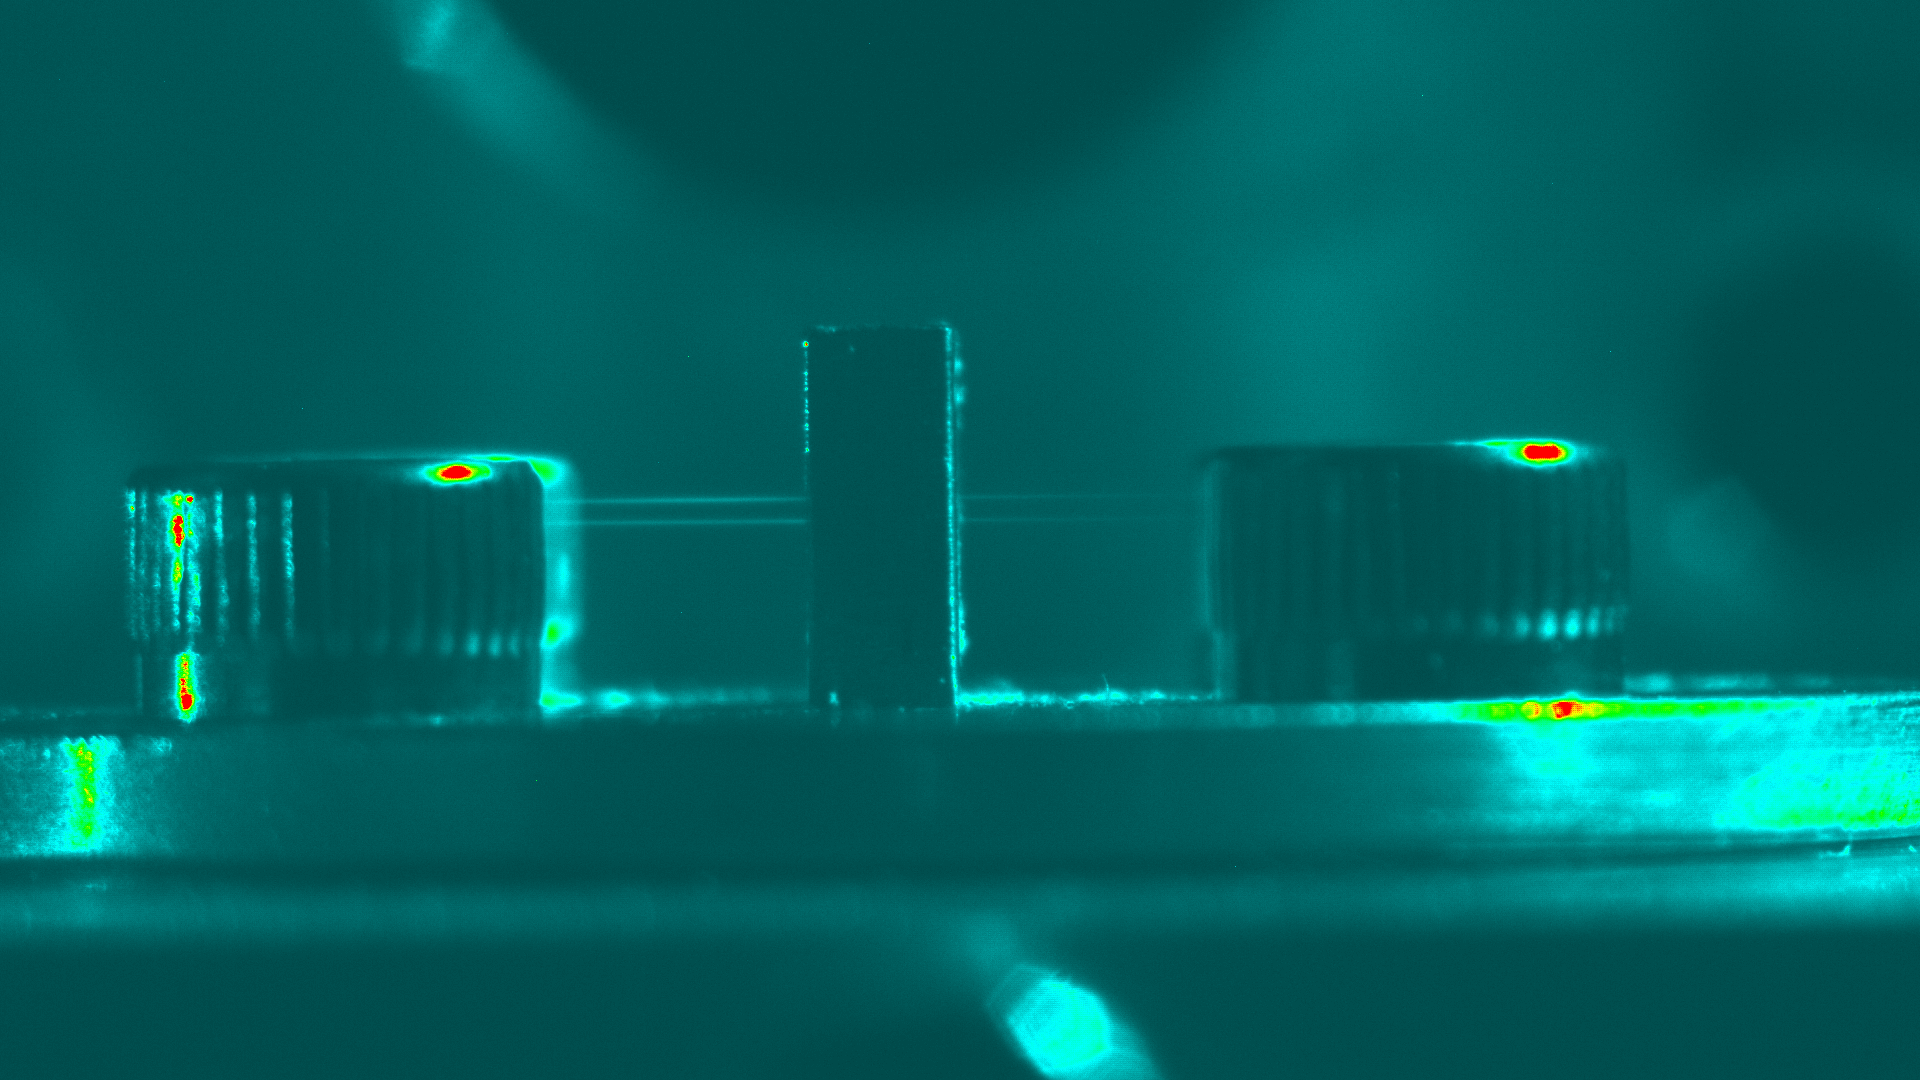
\includegraphics[width=0.9\textwidth]{figures/Two_source/ts_filament_gas_cell.png}
	\caption{Camera image of two sources generating a filament in a gas cell. Image was taken while chamber was vented and at ambient pressure.}
	\label{ts_filament}
\end{figure}

%\lipsum

\begin{figure}
	\centering
	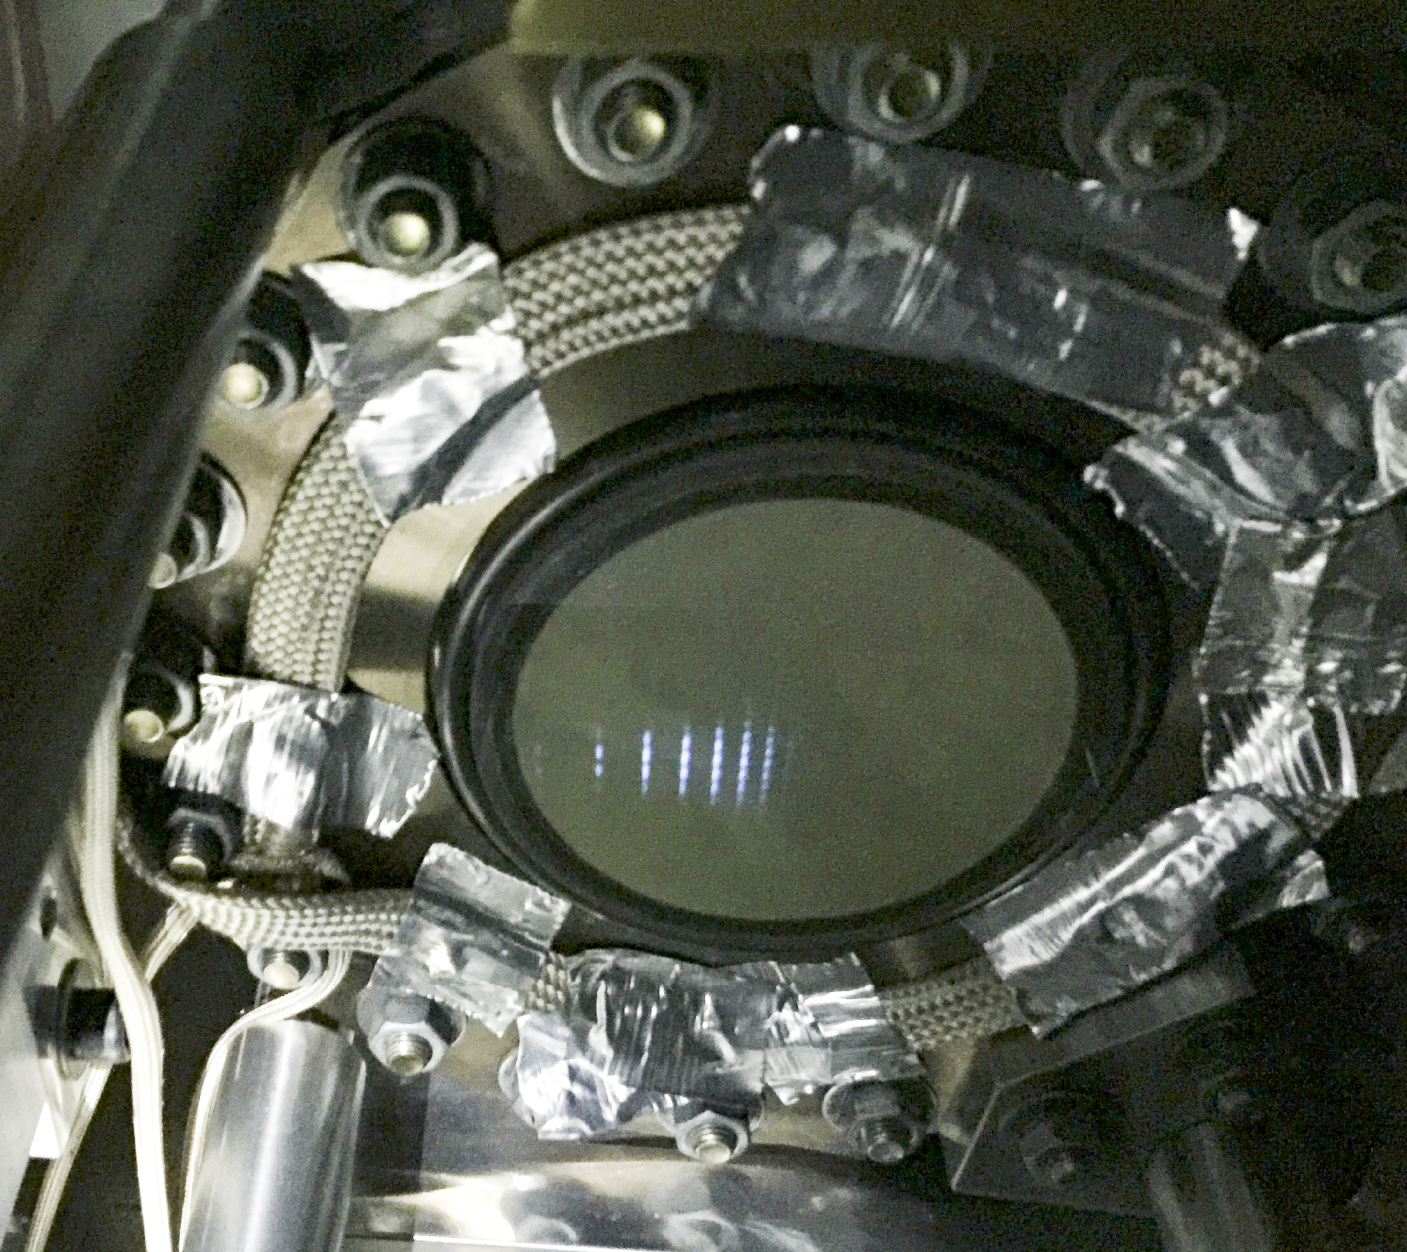
\includegraphics[width=0.9\textwidth]{figures/Two_source/MCP_ts_harmonics.png}
	\caption{Camera image of the output of the phosphor screen.  Harmonics are visible by eye.}
	\label{MCP_ts_harmonics}
\end{figure}


%\lipsum